\documentclass[parskip=half, bibliography=totoc, captions=tableheading, titlepage=firstiscover]{scrartcl}
\usepackage{polyglossia}
\setmainlanguage{german}

\usepackage{xcolor}
\xdefinecolor{tugreen}{RGB}{128, 186, 38}

\usepackage[pdfusetitle, unicode, allbordercolors = tugreen]{hyperref}

\usepackage{scrpage2}
\pagestyle{scrheadings}

%\usepackage{polyglossia}


\usepackage{caption}
\usepackage{subcaption}
\usepackage{amsmath}
\usepackage{amssymb}
\usepackage{mathtools}


\usepackage[autostyle]{csquotes}
\setdefaultlanguage{german}
\usepackage[
  locale=DE,                   % deutsche Einstellungen
  separate-uncertainty=true,   % Immer Fehler mit \pm
  per-mode=symbol-or-fraction, % m/s im Text, sonst Brüche
]{siunitx}

% von Julian eingefügt, weil der immer autoref benutzt
\AtBeginDocument{%
  \newcaptionname{ngerman}{\figureautorefname}{Abbildung}
  \newcaptionname{ngerman}{\tableautorefname}{Tabelle}
  \newcaptionname{ngerman}{\sectionautorefname}{Kapitel}
  \newcaptionname{ngerman}{\subsectionautorefname}{Kapitel}
  \newcaptionname{ngerman}{\chapterautorefname}{Kapitel}%
}

\usepackage{xfrac}

\usepackage[section, below]{placeins}
\usepackage[
  labelfont=bf,
  font=small,
  width=0.9\textwidth,
]{caption}


%\usepackage{subfig}

\usepackage{graphicx}

\usepackage{sidecap}  % von julian für sidecaptionseingefügt

\usepackage{float}
\floatplacement{figure}{h}
\floatplacement{table}{h}

\usepackage{booktabs}



\usepackage{bookmark}

\usepackage[shortcuts]{extdash}

\usepackage[math]{blindtext}

%\usepackage{microtype}

\usepackage[
  backend=biber,   % use modern biber backend
  autolang=hyphen,  % load hyphenation rules for if language of bibentry is not % in the references.bib use langid={en} for english sources
  sortcites = none,
  sorting = none,
]{biblatex}
% Quellendatenbank
\addbibresource{lit.bib}




\usepackage{makeidx}
\makeindex

\usepackage[version=3]{mhchem}
\usepackage{enumitem}
\usepackage{expl3}
\usepackage{xparse}

\RequirePackage{etoolbox}
\AtEndPreamble{
    \usepackage{fontspec}
    \usepackage{microtype}
    \usepackage{fontspec}
    \defaultfontfeatures{Ligatures=TeX}
    \usepackage{polyglossia}
    \setmainlanguage{german}
    \usepackage[
      math-style=ISO,
      bold-style=ISO,
      sans-style=italic,
      nabla=upright,
      ]{unicode-math}
    \setmathfont{Latin Modern Math}

}

\usepackage{yfonts}


%\usepackage{showframe}
\newcommand{\map}[1]{\mathup{#1}}
\newcommand{\ua}[1]{_{\mathup{#1}}}
\newcommand{\be}[1]{\left|\,#1\,\right|}
\newcommand{\norm}[1]{\|\,#1\,\|}
\newcommand{\ov}[1]{\overline{#1}}
\newcommand{\dv}[1]{\,\mathup{d}#1}
\newcommand{\tens}[1]{\underline{\underline{#1}}}
\NewDocumentCommand\dif{m}{\mathinner{\symup{d} #1}}
\newcommand{\versuch}{Nanoplasmonik und Dunkelfeldmikroskopie}
\newcommand{\vd}{Tag der Durchführung: 07.06.19}
\newcommand{\va}{Tag der Abgabe: }

\author{Julian Schröer \\
\href{mailto:julian.schroeer@tu-dortmund.de}{julian.schroeer@tu-dortmund.de} \\
und \\
Stefan Grisard \\
\href{mailto:stefan.grisard@tu-dortmund.de}{stefan.grisard@tu-dortmund.de}}
\title{\versuch}
\subtitle{Fortgeschrittenpraktikum 2, Festkörperphysik
\begin{figure}
  \centering
  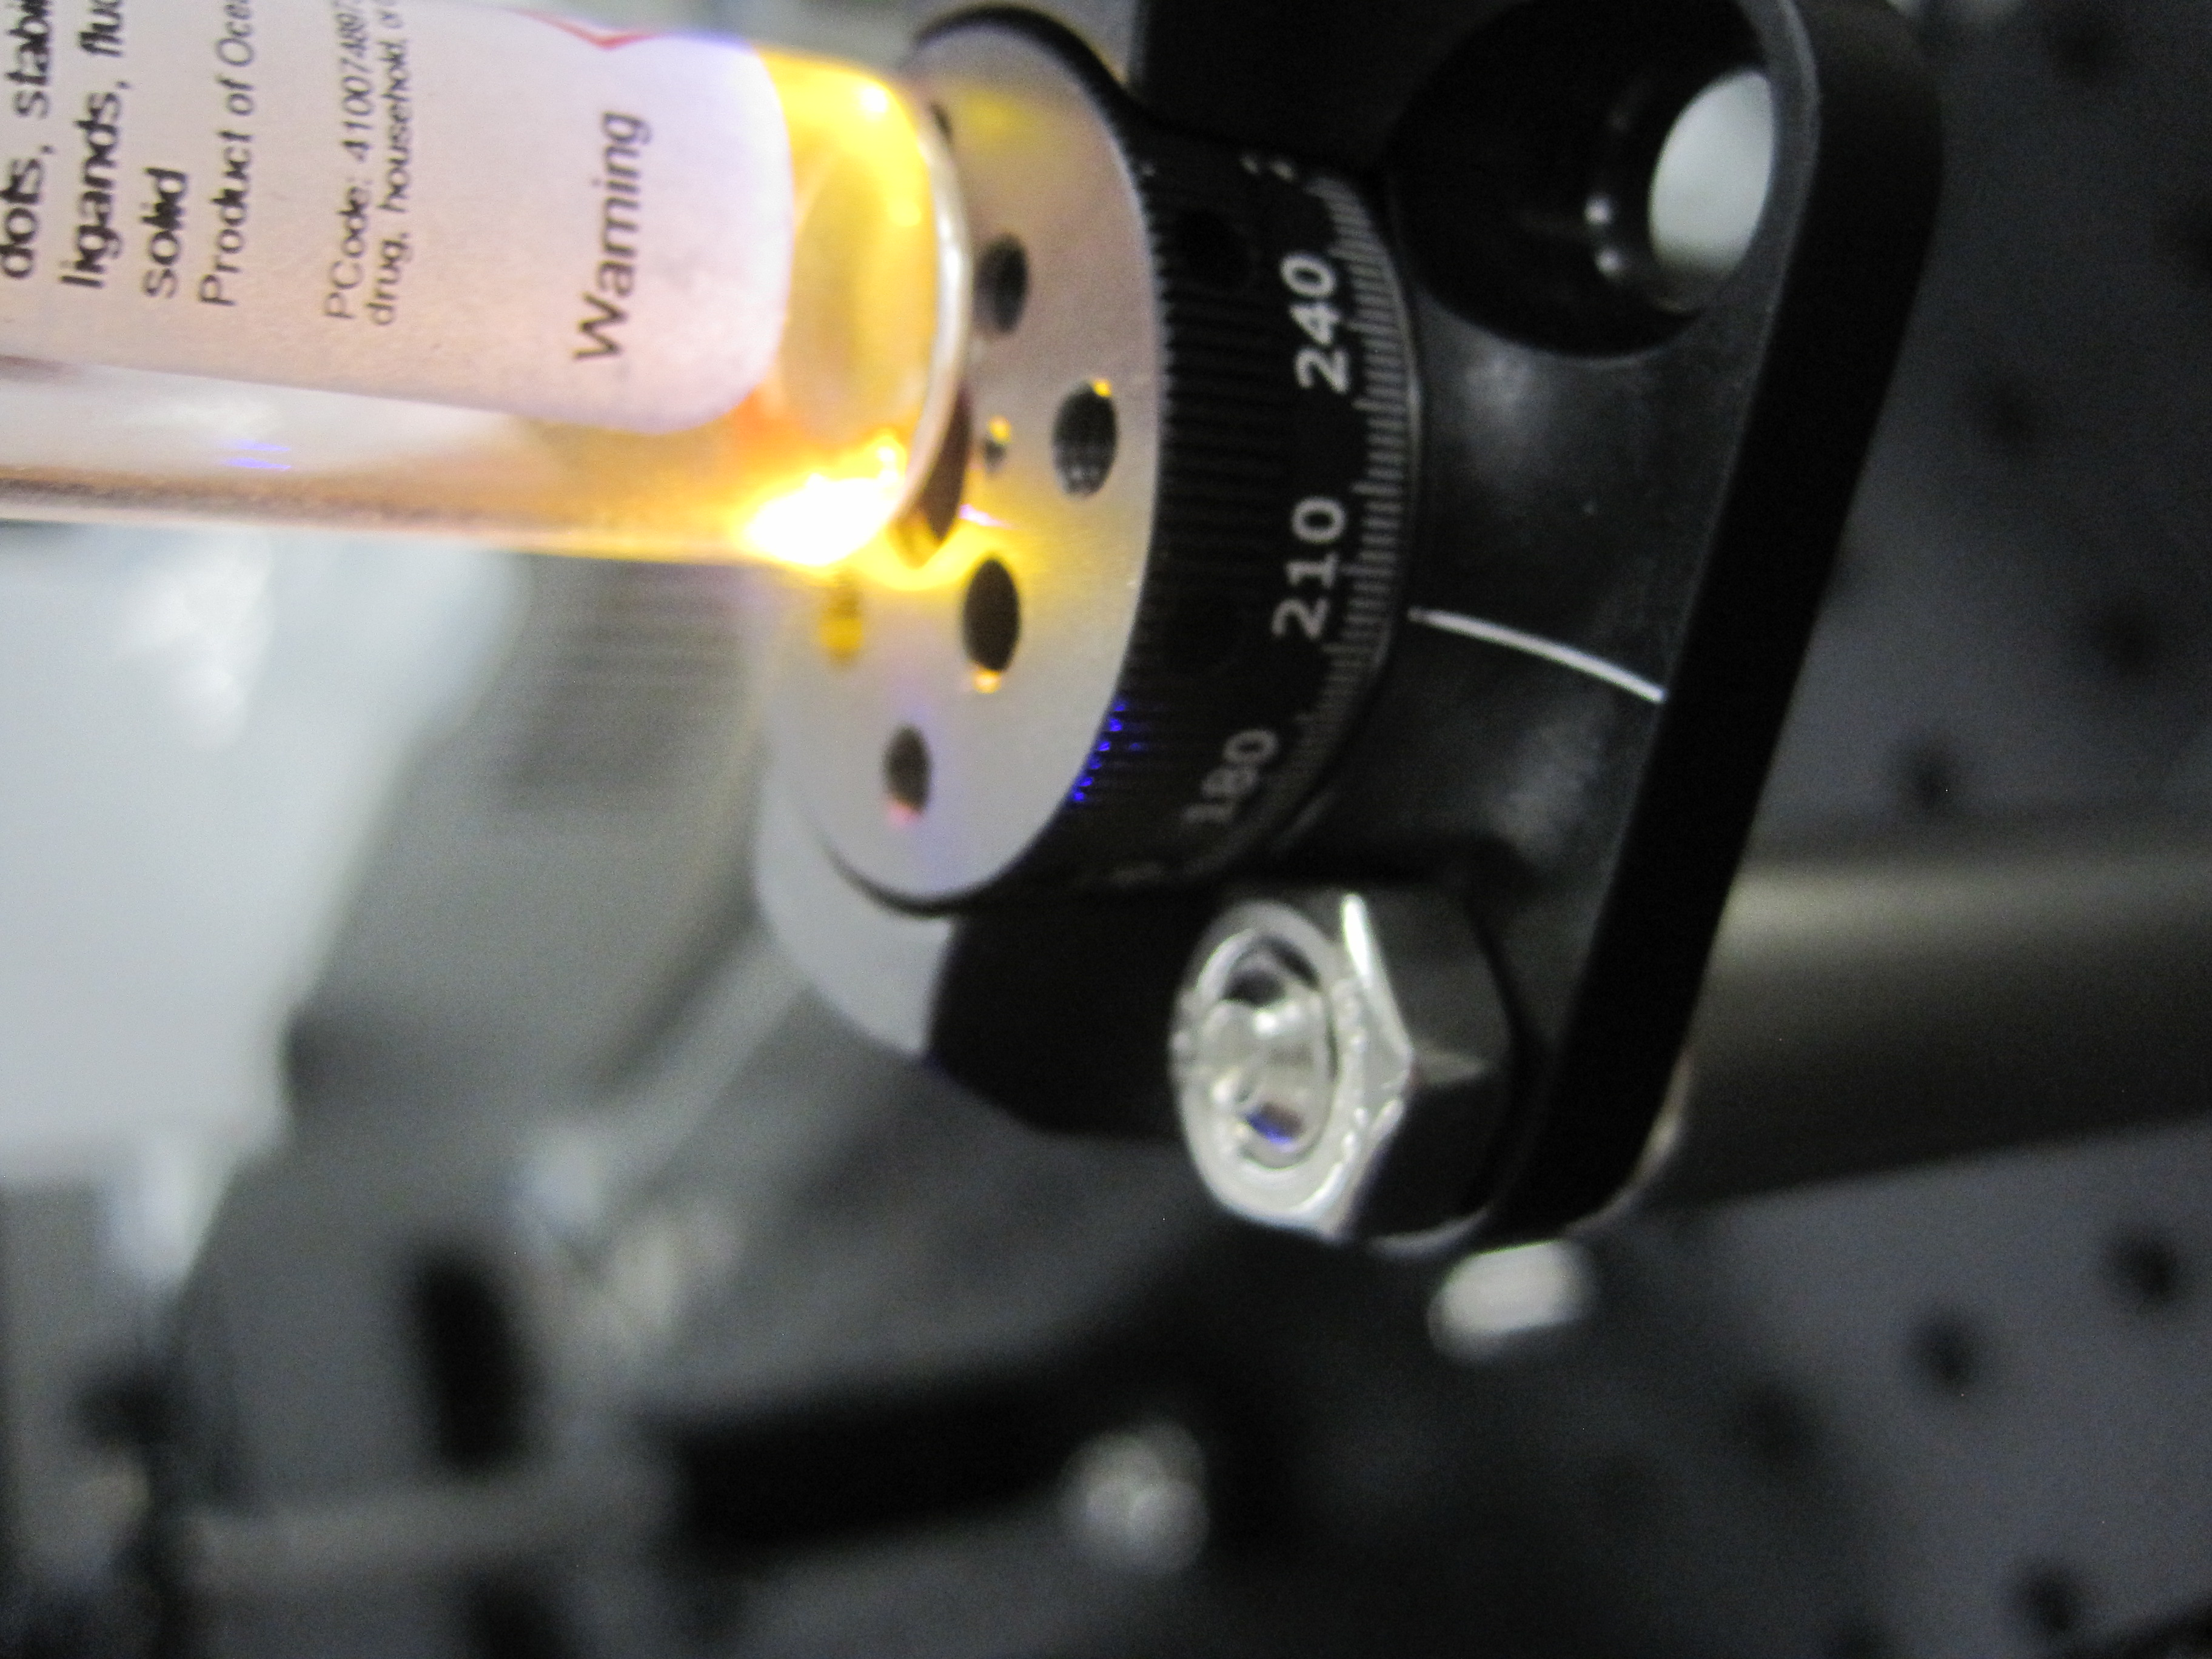
\includegraphics[width = 0.4\textwidth, angle = -90]{pics/title_pic.jpg}
\end{figure}
}
\date{\vd \\
\va}
\ohead{\today}
\cfoot{\pagemark}



%\usepackage{scrlayer-scrpage}
